\subsection*{Periodo per eventuale recupero e revisione}
Dal 24 Maggio al 13 Giugno si prevedono giorni di recupero per terminare la macrofase RTB e i giorni necessari ad effettuare il colloquio con i committenti.

\subsection{Product Baseline}
La macrofase Product Baseline è suddivisa in 4 incrementi che sono raggruppati in 2 fasi:
\begin{itemize}
    \item \textbf{Requisiti Obbligatori} dal 2022-06-13 al 2022-07-11;
            \begin{itemize}
                \item Incremento 1 dal 2022-06-13 al 2022-06-27;
                \item Incremento 2 dal 2022-06-28 al 2022-07-11;
            \end{itemize}
    \item \textbf{Requisiti Desiderabili} dal 2022-07-12 al 2022-07-25;
            \begin{itemize}
                \item Incremento 3 dal 2022-07-12 al 2022-07-18;
                \item Incremento 4 dal 2022-07-19 al 2022-07-25;
            \end{itemize}
\end{itemize}
Per la descrizione, corrispondenza tra i codici dei casi d'uso e i requisiti si faccia riferimento al documento Analisi dei Requisiti {\docVersionAdR}. \newline
Per ogni implementazione di una funzionalità il progettista progetta, il programmatore scrive il codice implementandola e il verificatore esegue i test di controllo segnalando gli eventuali errori / bug.
\subsubsection{Requisiti Obbligatori}
\paragraph{Incremento 1}
\begin{itemize}
    \item \textbf{Implementazione input testuale e vocale:} RO-F-1, 2, 61;
    \item \textbf{Implementazione autenticazione mediante \glossario{token}:} RO-F-3 a 6, 51, 52, 57 (UC1, UC13, UC18);
    \item \textbf{Implementazione gestione comandi non validi ed errori:} RO-F-8, 9, da 47 a 50 (UC2, UC10, UC11, UC12);
    \item \textbf{Specifica Architetturale, Manuale Utente:} creazione e inizio scrittura dei documenti con progettista e programmatore. La Specifica Architetturale illustrerà l'architettura del prodotto, mentre il Manuale Utente fornirà le istruzioni necessarie per l'uso del \glossario{chatbot};
    \item \textbf{Verifica:} il verificatore controlla che siano state rispettate le norme e verifica il materiale scritto e il prodotto realizzato durante questa fase;
    \item \textbf{Checkpoint:} per la descrizione dettagliata si veda \$4.1.2;
\end{itemize}

\paragraph{Incremento 2}
\begin{itemize}
    \item \textbf{Implementazione della registrazione presenza:} RO-F-10 a 12, 46, 60 (UC3, UC9, UC20);
    \item \textbf{Implementazione della consuntivazione:} RO-F-13 a 21, 53, 54, 62 (UC4, UC14, UC15, UC21);
    \item \textbf{Specifica Architetturale, Manuale Utente:} continua la scrittura dei documenti con progettista e programmatore;
    \item \textbf{Verifica:} il verificatore controlla che siano state rispettate le norme e verifica il materiale scritto e il prodotto realizzato durante questa fase;
    \item \textbf{Checkpoint:} per la descrizione dettagliata si veda \$4.1.2;
\end{itemize}

\begin{landscape}
	\begin{figure}
	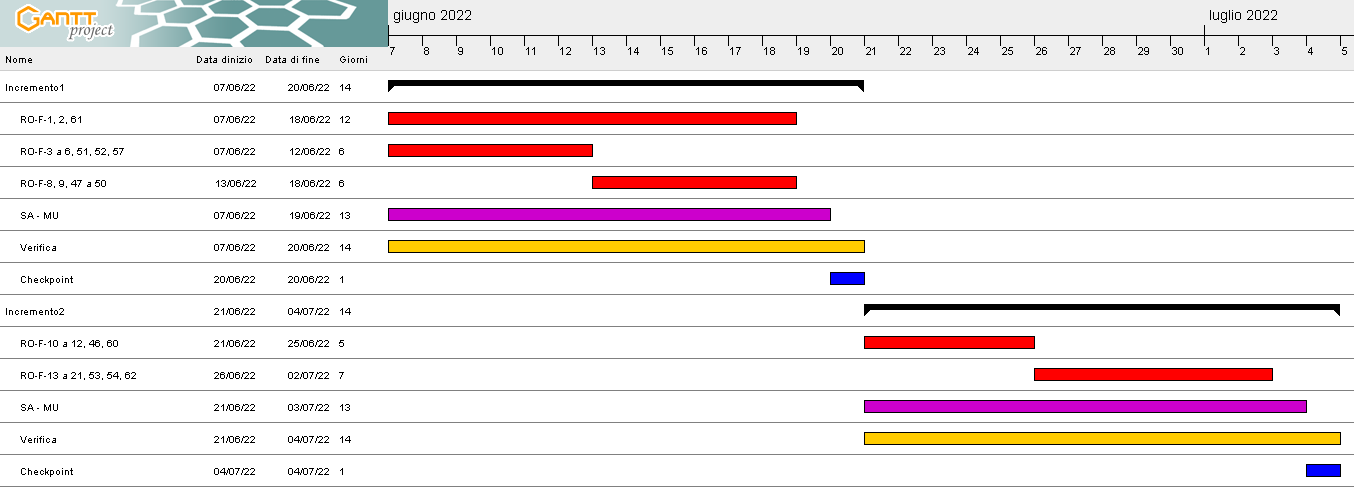
\includegraphics[width=\linewidth]{images/PB_obbligatori.png}
    \caption{Diagramma di Gantt - Macrofase PB, fase Requisiti Obbligatori}
	\end{figure}
\end{landscape}

\subsubsection{Requisiti Desiderabili}
\paragraph{Incremento 3}
\begin{itemize}
    \item \textbf{Implementazione autenticazione a scelta tra più \glossario{token}:} RD-F-7;
    \item \textbf{Implementazione della creazione di riunioni:} RD-F-24 a 32, 56, 58, 59 (UC6, UC17, UC19);
    \item \textbf{Implementazione dell'apertura del cancello:} RO-F-22, 23 (UC5);
    \item \textbf{Specifica Architetturale, Manuale Utente:} continua la scrittura dei documenti con progettista e programmatore;
    \item \textbf{Verifica:} il verificatore controlla che siano state rispettate le norme e verifica il materiale scritto e il prodotto realizzato durante questa fase;
    \item \textbf{Checkpoint:} per la descrizione dettagliata si veda \$4.1.2;
\end{itemize}

\paragraph{Incremento 4}
\begin{itemize}
    \item \textbf{Implementazione della ricerca di documenti:} RO-F-33 a 37, 55 (UC7, UC16);
    \item \textbf{Implementazione dell'inserimento di \glossario{ticket}:} RO-F-38 a 45 (UC8);
    \item \textbf{Specifica Architetturale, Manuale Utente:} termina la scrittura dei documenti;
    \item \textbf{Verifica:} il verificatore controlla che siano state rispettate le norme e verifica il materiale scritto e il prodotto realizzato durante questa fase;
    \item \textbf{Approvazione:} il responsabile controlla, approva il materiale e il prodotto realizzato durante questa macrofase PB;
    \item \textbf{Checkpoint:} per la descrizione dettagliata si veda \$4.1.2;
    \item \textbf{Presentazione PB:} viene preparata la presentazione per il colloquio e pubblicato il materiale nella repository pubblica e nel branch main.
\end{itemize}

\begin{landscape}
	\begin{figure}
	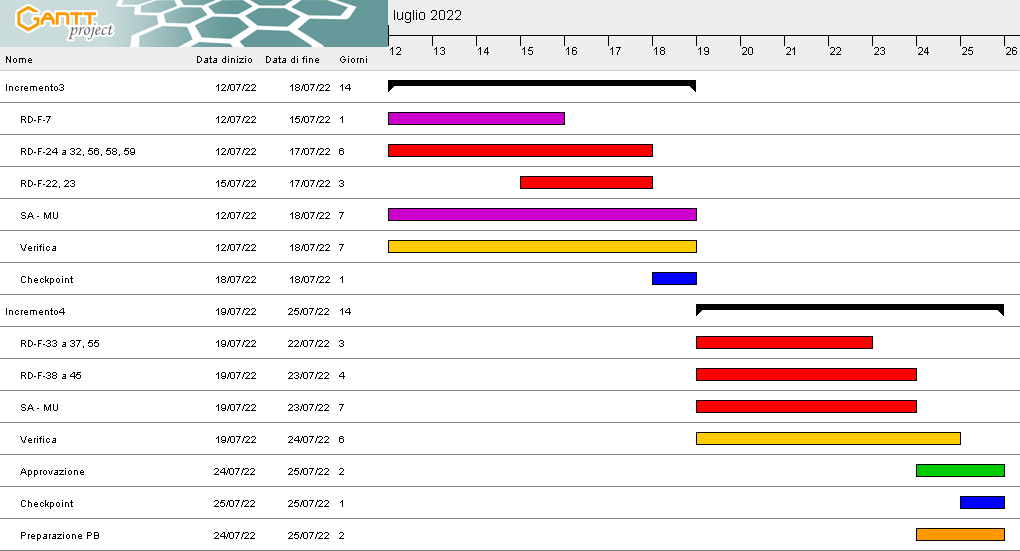
\includegraphics[width=\linewidth]{images/PB_desiderabili.png}
    \caption{Diagramma di Gantt - Macrofase PB, fase Requisiti Desiderabili}
	\end{figure}
\end{landscape}

\begin{landscape}
	\begin{figure}
	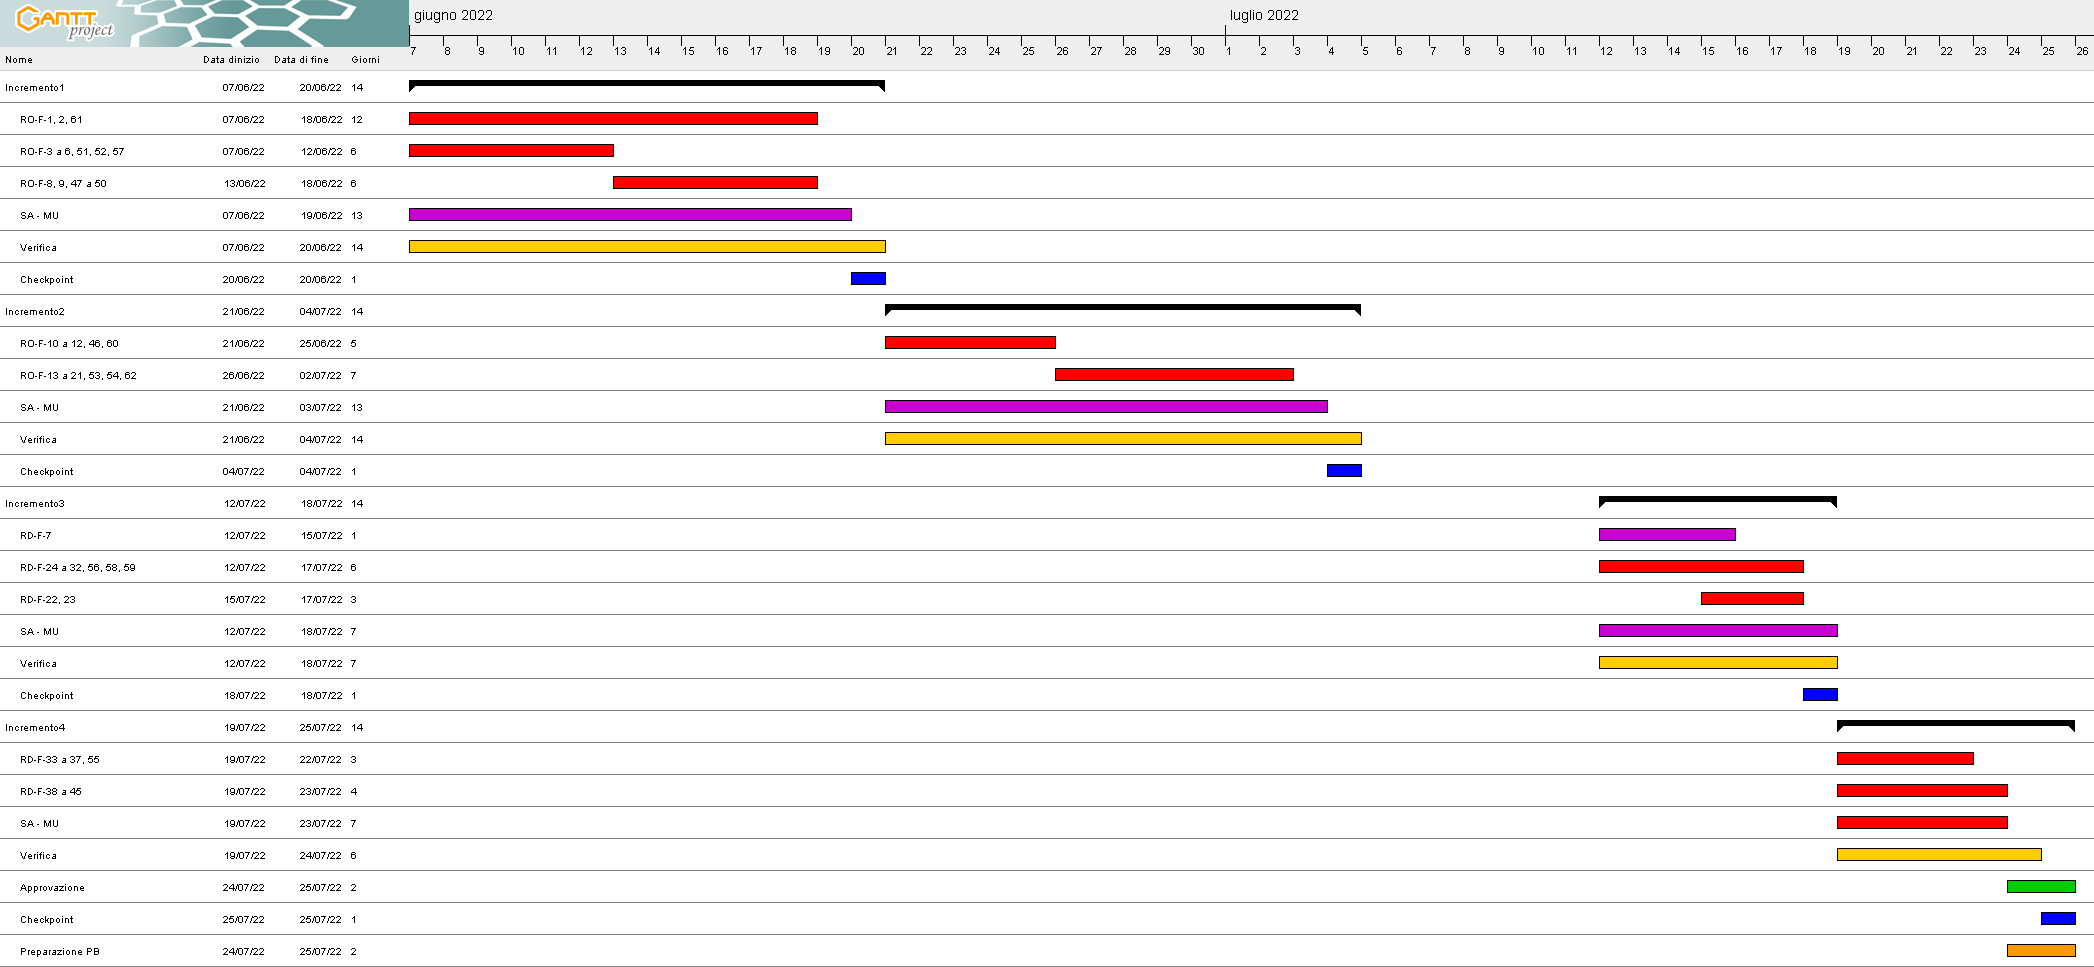
\includegraphics[width=\linewidth]{images/PB.png}
    \caption{Diagramma di Gantt - Macrofase PB}
	\end{figure}
\end{landscape}

\newpage